\documentclass{beamer}
%\documentclass[xcolor=pst,dvips,epic,eepic]{beamer}

\usepackage[utf8]{inputenc}
\usetheme{Singapore}
\usepackage{xcolor}
\setbeamertemplate{footline}[frame number]

\usepackage{mathlist}

\usepackage{amsmath,amssymb, amsthm}
\usepackage{amscd}

%\newtheorem{theo}{Théorème}

\usepackage{pstricks, pst-node}

\usepackage{times}

\usepackage{ulem}

\usepackage{listings}
%\topmargin=-0.6in
\lstloadlanguages{C++}
\lstset{language=C++}
%%}

\setbeamercovered{dynamic}

% We add the following commonly used macros:

% vectors as boldsymbols:
\newcommand{\bsa}{{\boldsymbol{a}}}
\newcommand{\bsb}{{\boldsymbol{b}}}
\newcommand{\bsc}{{\boldsymbol{c}}}
\newcommand{\bsd}{{\boldsymbol{d}}}
\newcommand{\bse}{{\boldsymbol{e}}}
\newcommand{\bsf}{{\boldsymbol{f}}}
\newcommand{\bsg}{{\boldsymbol{g}}}
\newcommand{\bsh}{{\boldsymbol{h}}}
\newcommand{\bsi}{{\boldsymbol{i}}}
\newcommand{\bsj}{{\boldsymbol{j}}}
\newcommand{\bsk}{{\boldsymbol{k}}}
\newcommand{\bsl}{{\boldsymbol{l}}}
\newcommand{\bsm}{{\boldsymbol{m}}}
\newcommand{\bsn}{{\boldsymbol{n}}}
\newcommand{\bso}{{\boldsymbol{o}}}
\newcommand{\bsp}{{\boldsymbol{p}}}
\newcommand{\bsq}{{\boldsymbol{q}}}
\newcommand{\bsr}{{\boldsymbol{r}}}
\newcommand{\bss}{{\boldsymbol{s}}}
\newcommand{\bst}{{\boldsymbol{t}}}
\newcommand{\bsu}{{\boldsymbol{u}}}
\newcommand{\bsv}{{\boldsymbol{v}}}
\newcommand{\bsw}{{\boldsymbol{w}}}
\newcommand{\bsx}{{\boldsymbol{x}}}
\newcommand{\bsy}{{\boldsymbol{y}}}
\newcommand{\bsz}{{\boldsymbol{z}}}
\newcommand{\bsA}{{\boldsymbol{A}}}
\newcommand{\bsB}{{\boldsymbol{B}}}
\newcommand{\bsC}{{\boldsymbol{C}}}
\newcommand{\bsD}{{\boldsymbol{D}}}
\newcommand{\bsE}{{\boldsymbol{E}}}
\newcommand{\bsF}{{\boldsymbol{F}}}
\newcommand{\bsG}{{\boldsymbol{G}}}
\newcommand{\bsH}{{\boldsymbol{H}}}
\newcommand{\bsI}{{\boldsymbol{I}}}
\newcommand{\bsJ}{{\boldsymbol{J}}}
\newcommand{\bsK}{{\boldsymbol{K}}}
\newcommand{\bsL}{{\boldsymbol{L}}}
\newcommand{\bsM}{{\boldsymbol{M}}}
\newcommand{\bsN}{{\boldsymbol{N}}}
\newcommand{\bsO}{{\boldsymbol{O}}}
\newcommand{\bsP}{{\boldsymbol{P}}}
\newcommand{\bsQ}{{\boldsymbol{Q}}}
\newcommand{\bsR}{{\boldsymbol{R}}}
\newcommand{\bsS}{{\boldsymbol{S}}}
\newcommand{\bsT}{{\boldsymbol{T}}}
\newcommand{\bsU}{{\boldsymbol{U}}}
\newcommand{\bsV}{{\boldsymbol{V}}}
\newcommand{\bsW}{{\boldsymbol{W}}}
\newcommand{\bsX}{{\boldsymbol{X}}}
\newcommand{\bsY}{{\boldsymbol{Y}}}
\newcommand{\bsZ}{{\boldsymbol{Z}}}
% other commonly used boldsymbols:
\newcommand{\bsell}{{\boldsymbol{\ell}}}
\newcommand{\bszero}{{\boldsymbol{0}}} % vector of zeros
\newcommand{\bsone}{{\boldsymbol{1}}}  % vector of ones
% boldsymbol greeks:
\newcommand{\bsalpha}{{\boldsymbol{\alpha}}}
\newcommand{\bsbeta}{{\boldsymbol{\beta}}}
\newcommand{\bsgamma}{{\boldsymbol{\gamma}}}
\newcommand{\bsdelta}{{\boldsymbol{\delta}}}
\newcommand{\bsepsilon}{{\boldsymbol{\epsilon}}}
\newcommand{\bsvarepsilon}{{\boldsymbol{\varepsilon}}}
\newcommand{\bszeta}{{\boldsymbol{\zeta}}}
\newcommand{\bseta}{{\boldsymbol{\eta}}}
\newcommand{\bstheta}{{\boldsymbol{\theta}}}
\newcommand{\bsvartheta}{{\boldsymbol{\vartheta}}}
\newcommand{\bskappa}{{\boldsymbol{\kappa}}}
\newcommand{\bslambda}{{\boldsymbol{\lambda}}}
\newcommand{\bsmu}{{\boldsymbol{\mu}}}
\newcommand{\bsnu}{{\boldsymbol{\nu}}}
\newcommand{\bsxi}{{\boldsymbol{\xi}}}
\newcommand{\bspi}{{\boldsymbol{\pi}}}
\newcommand{\bsvarpi}{{\boldsymbol{\varpi}}}
\newcommand{\bsrho}{{\boldsymbol{\rho}}}
\newcommand{\bsvarrho}{{\boldsymbol{\varrho}}}
\newcommand{\bssigma}{{\boldsymbol{\sigma}}}
\newcommand{\bsvarsigma}{{\boldsymbol{\varsigma}}}
\newcommand{\bstau}{{\boldsymbol{\tau}}}
\newcommand{\bsupsilon}{{\boldsymbol{\upsilon}}}
\newcommand{\bsphi}{{\boldsymbol{\phi}}}
\newcommand{\bsvarphi}{{\boldsymbol{\varphi}}}
\newcommand{\bschi}{{\boldsymbol{\chi}}}
\newcommand{\bspsi}{{\boldsymbol{\psi}}}
\newcommand{\bsomega}{{\boldsymbol{\omega}}}
\newcommand{\bsGamma}{{\boldsymbol{\Gamma}}}
\newcommand{\bsDelta}{{\boldsymbol{\Delta}}}
\newcommand{\bsTheta}{{\boldsymbol{\Theta}}}
\newcommand{\bsLambda}{{\boldsymbol{\Lambda}}}
\newcommand{\bsXi}{{\boldsymbol{\Xi}}}
\newcommand{\bsPi}{{\boldsymbol{\Pi}}}
\newcommand{\bsSigma}{{\boldsymbol{\Sigma}}}
\newcommand{\bsUpsilon}{{\boldsymbol{\Upsilon}}}
\newcommand{\bsPhi}{{\boldsymbol{\Phi}}}
\newcommand{\bsPsi}{{\boldsymbol{\Psi}}}
\newcommand{\bsOmega}{{\boldsymbol{\Omega}}}

% Roman fonts:
\newcommand{\rma}{{\mathrm{a}}}
\newcommand{\rmb}{{\mathrm{b}}}
\newcommand{\rmc}{{\mathrm{c}}}
\newcommand{\rmd}{{\mathrm{d}}}
\newcommand{\rme}{{\mathrm{e}}}
\newcommand{\rmf}{{\mathrm{f}}}
\newcommand{\rmg}{{\mathrm{g}}}
\newcommand{\rmh}{{\mathrm{h}}}
\newcommand{\rmi}{{\mathrm{i}}}
\newcommand{\rmj}{{\mathrm{j}}}
\newcommand{\rmk}{{\mathrm{k}}}
\newcommand{\rml}{{\mathrm{l}}}
\newcommand{\rmm}{{\mathrm{m}}}
\newcommand{\rmn}{{\mathrm{n}}}
\newcommand{\rmo}{{\mathrm{o}}}
\newcommand{\rmp}{{\mathrm{p}}}
\newcommand{\rmq}{{\mathrm{q}}}
\newcommand{\rmr}{{\mathrm{r}}}
\newcommand{\rms}{{\mathrm{s}}}
\newcommand{\rmt}{{\mathrm{t}}}
\newcommand{\rmu}{{\mathrm{u}}}
\newcommand{\rmv}{{\mathrm{v}}}
\newcommand{\rmw}{{\mathrm{w}}}
\newcommand{\rmx}{{\mathrm{x}}}
\newcommand{\rmy}{{\mathrm{y}}}
\newcommand{\rmz}{{\mathrm{z}}}
\newcommand{\rmA}{{\mathrm{A}}}
\newcommand{\rmB}{{\mathrm{B}}}
\newcommand{\rmC}{{\mathrm{C}}}
\newcommand{\rmD}{{\mathrm{D}}}
\newcommand{\rmE}{{\mathrm{E}}}
\newcommand{\rmF}{{\mathrm{F}}}
\newcommand{\rmG}{{\mathrm{G}}}
\newcommand{\rmH}{{\mathrm{H}}}
\newcommand{\rmI}{{\mathrm{I}}}
\newcommand{\rmJ}{{\mathrm{J}}}
\newcommand{\rmK}{{\mathrm{K}}}
\newcommand{\rmL}{{\mathrm{L}}}
\newcommand{\rmM}{{\mathrm{M}}}
\newcommand{\rmN}{{\mathrm{N}}}
\newcommand{\rmO}{{\mathrm{O}}}
\newcommand{\rmP}{{\mathrm{P}}}
\newcommand{\rmQ}{{\mathrm{Q}}}
\newcommand{\rmR}{{\mathrm{R}}}
\newcommand{\rmS}{{\mathrm{S}}}
\newcommand{\rmT}{{\mathrm{T}}}
\newcommand{\rmU}{{\mathrm{U}}}
\newcommand{\rmV}{{\mathrm{V}}}
\newcommand{\rmW}{{\mathrm{W}}}
\newcommand{\rmX}{{\mathrm{X}}}
\newcommand{\rmY}{{\mathrm{Y}}}
\newcommand{\rmZ}{{\mathrm{Z}}}
% also commonly defined
\newcommand{\rd}{{\mathrm{d}}}
\newcommand{\ri}{{\mathrm{i}}}

% blackboards:
\newcommand{\bbA}{{\mathbb{A}}}
\newcommand{\bbB}{{\mathbb{B}}}
\newcommand{\bbC}{{\mathbb{C}}}
\newcommand{\bbD}{{\mathbb{D}}}
\newcommand{\bbE}{{\mathbb{E}}}
\newcommand{\bbF}{{\mathbb{F}}}
\newcommand{\bbG}{{\mathbb{G}}}
\newcommand{\bbH}{{\mathbb{H}}}
\newcommand{\bbI}{{\mathbb{I}}}
\newcommand{\bbJ}{{\mathbb{J}}}
\newcommand{\bbK}{{\mathbb{K}}}
\newcommand{\bbL}{{\mathbb{L}}}
\newcommand{\bbM}{{\mathbb{M}}}
\newcommand{\bbN}{{\mathbb{N}}}
\newcommand{\bbO}{{\mathbb{O}}}
\newcommand{\bbP}{{\mathbb{P}}}
\newcommand{\bbQ}{{\mathbb{Q}}}
\newcommand{\bbR}{{\mathbb{R}}}
\newcommand{\bbS}{{\mathbb{S}}}
\newcommand{\bbT}{{\mathbb{T}}}
\newcommand{\bbU}{{\mathbb{U}}}
\newcommand{\bbV}{{\mathbb{V}}}
\newcommand{\bbW}{{\mathbb{W}}}
\newcommand{\bbX}{{\mathbb{X}}}
\newcommand{\bbY}{{\mathbb{Y}}}
\newcommand{\bbZ}{{\mathbb{Z}}}
% commonly used shortcuts:
\newcommand{\C}{{\mathbb{C}}} % complex numbers
\newcommand{\F}{{\mathbb{F}}} % field, finite field
\newcommand{\N}{{\mathbb{N}}} % natural numbers {1, 2, ...}
\newcommand{\Q}{{\mathbb{Q}}} % rationals
\newcommand{\R}{{\mathbb{R}}} % reals
\newcommand{\Z}{{\mathbb{Z}}} % integers
% more commonly used shortcuts:
\newcommand{\CC}{{\mathbb{C}}} % complex numbers
\newcommand{\FF}{{\mathbb{F}}} % field, finite field
\newcommand{\NN}{{\mathbb{N}}} % natural numbers {1, 2, ...}
\newcommand{\QQ}{{\mathbb{Q}}} % rationals
\newcommand{\RR}{{\mathbb{R}}} % reals
\newcommand{\ZZ}{{\mathbb{Z}}} % integers
% more commonly used shortcuts:
\newcommand{\EE}{{\mathbb{E}}}
\newcommand{\PP}{{\mathbb{P}}}
\newcommand{\TT}{{\mathbb{T}}}
\newcommand{\VV}{{\mathbb{V}}}
% and even more commonly used shortcuts:
\newcommand{\Complex}{{\mathbb{C}}}
\newcommand{\Integer}{{\mathbb{Z}}}
\newcommand{\Natural}{{\mathbb{N}}}
\newcommand{\Rational}{{\mathbb{Q}}}
\newcommand{\Real}{{\mathbb{R}}}

%%% Issue with miktex
% indicator boldface 1:
%\DeclareSymbolFont{bbold}{U}{bbold}{m}{n}
%\DeclareSymbolFontAlphabet{\mathbbold}{bbold}
%\newcommand{\ind}{{\mathbbold{1}}}
%\newcommand{\bbone}{{\mathbbold{1}}}


% calligraphic letters:
\newcommand{\cala}{{\mathcal{a}}}
\newcommand{\calb}{{\mathcal{b}}}
\newcommand{\calc}{{\mathcal{c}}}
\newcommand{\cald}{{\mathcal{d}}}
\newcommand{\cale}{{\mathcal{e}}}
\newcommand{\calf}{{\mathcal{f}}}
\newcommand{\calg}{{\mathcal{g}}}
\newcommand{\calh}{{\mathcal{h}}}
\newcommand{\cali}{{\mathcal{i}}}
\newcommand{\calj}{{\mathcal{j}}}
\newcommand{\calk}{{\mathcal{k}}}
\newcommand{\call}{{\mathcal{l}}}
\newcommand{\calm}{{\mathcal{m}}}
\newcommand{\caln}{{\mathcal{n}}}
\newcommand{\calo}{{\mathcal{o}}}
\newcommand{\calp}{{\mathcal{p}}}
\newcommand{\calq}{{\mathcal{q}}}
\newcommand{\calr}{{\mathcal{r}}}
\newcommand{\cals}{{\mathcal{s}}}
\newcommand{\calt}{{\mathcal{t}}}
\newcommand{\calu}{{\mathcal{u}}}
\newcommand{\calv}{{\mathcal{v}}}
\newcommand{\calw}{{\mathcal{w}}}
\newcommand{\calx}{{\mathcal{x}}}
\newcommand{\caly}{{\mathcal{y}}}
\newcommand{\calz}{{\mathcal{z}}}
\newcommand{\calA}{{\mathcal{A}}}
\newcommand{\calB}{{\mathcal{B}}}
\newcommand{\calC}{{\mathcal{C}}}
\newcommand{\calD}{{\mathcal{D}}}
\newcommand{\calE}{{\mathcal{E}}}
\newcommand{\calF}{{\mathcal{F}}}
\newcommand{\calG}{{\mathcal{G}}}
\newcommand{\calH}{{\mathcal{H}}}
\newcommand{\calI}{{\mathcal{I}}}
\newcommand{\calJ}{{\mathcal{J}}}
\newcommand{\calK}{{\mathcal{K}}}
\newcommand{\calL}{{\mathcal{L}}}
\newcommand{\calM}{{\mathcal{M}}}
\newcommand{\calN}{{\mathcal{N}}}
\newcommand{\calO}{{\mathcal{O}}}
\newcommand{\calP}{{\mathcal{P}}}
\newcommand{\calQ}{{\mathcal{Q}}}
\newcommand{\calR}{{\mathcal{R}}}
\newcommand{\calS}{{\mathcal{S}}}
\newcommand{\calT}{{\mathcal{T}}}
\newcommand{\calU}{{\mathcal{U}}}
\newcommand{\calV}{{\mathcal{V}}}
\newcommand{\calW}{{\mathcal{W}}}
\newcommand{\calX}{{\mathcal{X}}}
\newcommand{\calY}{{\mathcal{Y}}}
\newcommand{\calZ}{{\mathcal{Z}}}

% Euler fraks:
\newcommand{\fraka}{{\mathfrak{a}}}
\newcommand{\frakb}{{\mathfrak{b}}}
\newcommand{\frakc}{{\mathfrak{c}}}
\newcommand{\frakd}{{\mathfrak{d}}}
\newcommand{\frake}{{\mathfrak{e}}}
\newcommand{\frakf}{{\mathfrak{f}}}
\newcommand{\frakg}{{\mathfrak{g}}}
\newcommand{\frakh}{{\mathfrak{h}}}
\newcommand{\fraki}{{\mathfrak{i}}}
\newcommand{\frakj}{{\mathfrak{j}}}
\newcommand{\frakk}{{\mathfrak{k}}}
\newcommand{\frakl}{{\mathfrak{l}}}
\newcommand{\frakm}{{\mathfrak{m}}}
\newcommand{\frakn}{{\mathfrak{n}}}
\newcommand{\frako}{{\mathfrak{o}}}
\newcommand{\frakp}{{\mathfrak{p}}}
\newcommand{\frakq}{{\mathfrak{q}}}
\newcommand{\frakr}{{\mathfrak{r}}}
\newcommand{\fraks}{{\mathfrak{s}}}
\newcommand{\frakt}{{\mathfrak{t}}}
\newcommand{\fraku}{{\mathfrak{u}}}
\newcommand{\frakv}{{\mathfrak{v}}}
\newcommand{\frakw}{{\mathfrak{w}}}
\newcommand{\frakx}{{\mathfrak{x}}}
\newcommand{\fraky}{{\mathfrak{y}}}
\newcommand{\frakz}{{\mathfrak{z}}}
\newcommand{\frakA}{{\mathfrak{A}}}
\newcommand{\frakB}{{\mathfrak{B}}}
\newcommand{\frakC}{{\mathfrak{C}}}
\newcommand{\frakD}{{\mathfrak{D}}}
\newcommand{\frakE}{{\mathfrak{E}}}
\newcommand{\frakF}{{\mathfrak{F}}}
\newcommand{\frakG}{{\mathfrak{G}}}
\newcommand{\frakH}{{\mathfrak{H}}}
\newcommand{\frakI}{{\mathfrak{I}}}
\newcommand{\frakJ}{{\mathfrak{J}}}
\newcommand{\frakK}{{\mathfrak{K}}}
\newcommand{\frakL}{{\mathfrak{L}}}
\newcommand{\frakM}{{\mathfrak{M}}}
\newcommand{\frakN}{{\mathfrak{N}}}
\newcommand{\frakO}{{\mathfrak{O}}}
\newcommand{\frakP}{{\mathfrak{P}}}
\newcommand{\frakQ}{{\mathfrak{Q}}}
\newcommand{\frakR}{{\mathfrak{R}}}
\newcommand{\frakS}{{\mathfrak{S}}}
\newcommand{\frakT}{{\mathfrak{T}}}
\newcommand{\frakU}{{\mathfrak{U}}}
\newcommand{\frakV}{{\mathfrak{V}}}
\newcommand{\frakW}{{\mathfrak{W}}}
\newcommand{\frakX}{{\mathfrak{X}}}
\newcommand{\frakY}{{\mathfrak{Y}}}
\newcommand{\frakZ}{{\mathfrak{Z}}}
% sets as Euler fraks:
\newcommand{\seta}{{\mathfrak{a}}}
\newcommand{\setb}{{\mathfrak{b}}}
\newcommand{\setc}{{\mathfrak{c}}}
\newcommand{\setd}{{\mathfrak{d}}}
\newcommand{\sete}{{\mathfrak{e}}}
\newcommand{\setf}{{\mathfrak{f}}}
\newcommand{\setg}{{\mathfrak{g}}}
\newcommand{\seth}{{\mathfrak{h}}}
\newcommand{\seti}{{\mathfrak{i}}}
\newcommand{\setj}{{\mathfrak{j}}}
\newcommand{\setk}{{\mathfrak{k}}}
\newcommand{\setl}{{\mathfrak{l}}}
\newcommand{\setm}{{\mathfrak{m}}}
\newcommand{\setn}{{\mathfrak{n}}}
\newcommand{\seto}{{\mathfrak{o}}}
\newcommand{\setp}{{\mathfrak{p}}}
\newcommand{\setq}{{\mathfrak{q}}}
\newcommand{\setr}{{\mathfrak{r}}}
\newcommand{\sets}{{\mathfrak{s}}}
\newcommand{\sett}{{\mathfrak{t}}}
\newcommand{\setu}{{\mathfrak{u}}}
\newcommand{\setv}{{\mathfrak{v}}}
\newcommand{\setw}{{\mathfrak{w}}}
\newcommand{\setx}{{\mathfrak{x}}}
\newcommand{\sety}{{\mathfrak{y}}}
\newcommand{\setz}{{\mathfrak{z}}}
\newcommand{\setA}{{\mathfrak{A}}}
\newcommand{\setB}{{\mathfrak{B}}}
\newcommand{\setC}{{\mathfrak{C}}}
\newcommand{\setD}{{\mathfrak{D}}}
\newcommand{\setE}{{\mathfrak{E}}}
\newcommand{\setF}{{\mathfrak{F}}}
\newcommand{\setG}{{\mathfrak{G}}}
\newcommand{\setH}{{\mathfrak{H}}}
\newcommand{\setI}{{\mathfrak{I}}}
\newcommand{\setJ}{{\mathfrak{J}}}
\newcommand{\setK}{{\mathfrak{K}}}
\newcommand{\setL}{{\mathfrak{L}}}
\newcommand{\setM}{{\mathfrak{M}}}
\newcommand{\setN}{{\mathfrak{N}}}
\newcommand{\setO}{{\mathfrak{O}}}
\newcommand{\setP}{{\mathfrak{P}}}
\newcommand{\setQ}{{\mathfrak{Q}}}
\newcommand{\setR}{{\mathfrak{R}}}
\newcommand{\setS}{{\mathfrak{S}}}
\newcommand{\setT}{{\mathfrak{T}}}
\newcommand{\setU}{{\mathfrak{U}}}
\newcommand{\setV}{{\mathfrak{V}}}
\newcommand{\setW}{{\mathfrak{W}}}
\newcommand{\setX}{{\mathfrak{X}}}
\newcommand{\setY}{{\mathfrak{Y}}}
\newcommand{\setZ}{{\mathfrak{Z}}}

% other commonly defined commands:
\newcommand{\wal}{{\rm wal}}
\newcommand{\floor}[1]{\left\lfloor #1 \right\rfloor} % floor
\newcommand{\ceil}[1]{\left\lceil #1 \right\rceil}    % ceil
\DeclareMathOperator{\cov}{Cov}
\DeclareMathOperator{\var}{Var}
\providecommand{\argmin}{\operatorname*{argmin}}
\providecommand{\argmax}{\operatorname*{argmax}}

\def\bxi{\boldsymbol\xi}
\def\bomega{\boldsymbol\omega}
\def\bC{\boldsymbol{C}}
\def\bu{\boldsymbol{u}}
\def\bU{\boldsymbol{U}}
\def\bu{\boldsymbol{u}}
\def\by{\boldsymbol{y}}
\def\vol{\mbox{vol}}

\title[Random Numbers Generation]{A short tutorial of random numbers generation}

\author[Fabian Bastin]{Fabian Bastin \\ \url{fabian.bastin@umontreal.ca} \\ Université de Montréal -- CIRRELT -- IVADO -- Fin-ML}
\date{}

\begin{document}
	
\titlegraphic{\vspace{-0.5cm}
	
\includegraphics[scale=0.2]{imgs/udem.png}
	\hspace{2cm}
	\includegraphics[scale=0.07]{imgs/Fin-MLLogo.png}
}
	\frame{\titlepage}
	
\begin{frame}
	%\frametitle{Outline}
	%

\begin{center}
	\href{https://xkcd.com/221/}{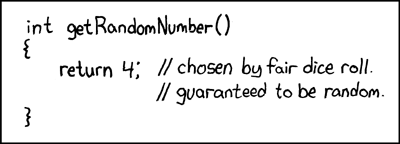
\includegraphics[scale=0.75]{imgs/random_number.png}}
\begin{small}
	\url{https://xkcd.com/221/}
\end{small}
\end{center}


%\begin{center}

%	\href{https://xkcd.com/221/}{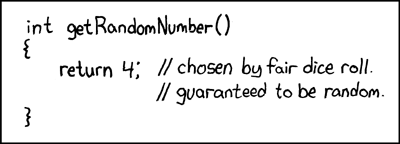
\includegraphics[scale=0.75]{imgs/random_number.png}}
%	\begin{small}
%		\url{https://xkcd.com/221/}
%	\end{small}

%\end{center}

\end{frame}
	
	\begin{frame}
		\frametitle{U[0,1]-distributed random numbers}
		
		\begin{itemize}
			\item
			A good uniform random generator on the interval $[0,1]$ is a major
			component of any good random generator library.
			\item
			Draws from other distributions are usually obtained by adequately transform an
			uniformly distributed sample.
		\end{itemize}
		
		\mbox{}
		
		Define a {\blue transition function} $f: \mathcal{S} \rightarrow \mathcal{S}$,
		where $\mathcal{S}$ is the {\blue state space}.
		The cardinality of $\mathcal{S}$ is assumed to be finite.
		
		\mbox{}
		
		The initial state is denoted by $s_0$, and we will write
		\[
		s_n = f(s_{n-1}).
		\]
		We will furthermore assume that $f$ is periodic for all $n$ greater of
		equal to some known $\tau$ (often equal to 0), with period $\rho$:
		$$
		s_{n+\rho} = s_n,\ \forall\, n\ge\tau.
		$$
		
	\end{frame}
	
	\begin{frame}
		\frametitle{U[0,1]-distributed random numbers (cont'd)}
		
		\begin{itemize}
			\item
			Output space: $\mathcal{U}$.
			\item
			We assume here that $\mathcal{U} = (0,1)$.
			\item
			Output function $g: \mathcal{S} \rightarrow \mathcal{U}$.\\
			It transforms the state $s_n$ into an output value $u_n$.
		\end{itemize}
		
		\begin{small}
			\[
			\begin{CD}
				\cdots @>f>> s_{\rho-1} @>f>> s_0 @>f>> s_1  @>f>> 
				\cdots @>f>> s_n @>f>> \cdots \\ 
				%
				@. @V{g}VV  @V{g}VV   @V{g}VV   
				@.  @V{g}VV  \\
				%
				\cdots @. u_{\rho-1} @. u_0
				@.  u_1  @.   \cdots @.  u_n @.  \cdots \\
			\end{CD}
			\]
			\label{fig:rng}
		\end{small}
		
		\mbox{}
		
		{\bf How to choose $f$ and $g$?}
		
		\mbox{}
		
		\textcolor{red}{Goals:} large $\rho$, good uniformity, ``random'' behavior.
		
	\end{frame}
	
	\begin{frame}
		\frametitle{Linear congruential generators (LCGs)}
		
\begin{itemize}
\item
Introduced by Lehmer (1951).
\item
State $s = x \in \NN_{\geq 0}$.
\item
Recursive formula:
$$
x_i = f(x_{i-1}) = (ax_{i-1}+c) \mod m,
$$
where $\mod$ is the modulo operator.\\
Given two numbers, a (the dividend) and n (the divisor),
$$
a \mod n = a - n\left\lfloor \frac{a}{n} \right\rfloor.
$$
\item
If $c = 0$, the generator is often called a multiplicative congruential generator, or ``{\red Lehmer RNG}''
\end{itemize}
		
\end{frame}
	
	\begin{frame}
		\frametitle{Linear congruential generators: full period?}
		
		Full period: $m$ is $c \ne 0$, $m-1$ otherwise (if $c = 0$, 0 is a
		fixed point for the recurrence).
		Consider the case $c \ne 0$.
		
		\begin{theorem}[Period]
			The LCG has full period iff the
			following three conditions hold:
			\begin{enumerate}
				\item
				the only positive integer that (exactly) divides both $m$ and $c$ is
				1;
				\item
				if $q$ is a prime number that divides $m$, then $q$ divides $a-1$;
				\item
				if 4 divides $m$, then 4 divides a-1.
			\end{enumerate}
		\end{theorem}
		``{\red Standard minimal}'' (Park and Miller, 1988):
		\[
		x_{n+1} = 16807x_n \mbox{ mod } 2147483647.
		\]
		Observe that $2147483647 = 2^{31}-1$; on 32-bit architectures, the
		largest representable (signed) integer is $2^{31}$.
		
	\end{frame}
	
	\begin{frame}[containsverbatim]
		\frametitle{The Standard Minimal Generator}
		
		\begin{small}
			\begin{verbatim}
function getlcg(seed::Integer, a::Integer,
                 c::Integer, m::Integer)
    state = seed
    am_mil = 1.0/m
    return function lcgrand()
        state = mod(a * state + c, m)
        # produce a number in (0,1)
        return state*am_mil
    end
end

stdmin = getlcg(1234, 16807, 0, 2^31-1)
		\end{verbatim}
		\end{small}
		
	\end{frame}
	
	\begin{frame}
		\frametitle{Standard minimal generator: illustration}
		\begin{center}
			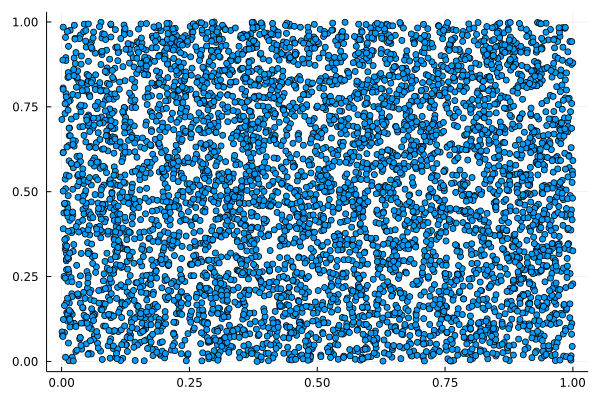
\includegraphics[width=0.8\linewidth]{imgs/lcg.png}
			
			10000 generated points on the unit square.
		\end{center}
		
	\end{frame}
	
	\begin{frame}
		\frametitle{Multiple Recursive Generator (MRG)}
		
		But we want better! Generalize the LCG:
		\[
		x_n = (a_1 x_{n-1} + \cdots + a_k x_{n-k}) \mod {m}, \quad  
		u_n = x_n / m.
		\]
		In practice, take $u_n = (x_n + 1) / (m+1)$, or $u_n =
		x_n/(m+1)$ if $x_n>0$ and $u_n = m/(m+1)$ otherwise, but the structure
		remains the same, and is easier when studying theoretical properties.
%		This kind of generators is very popular.
		
		\mbox{}
		
		State at step $n$:
		\[
		s_n = (x_{n-k+1},\dots,x_n)^T.
		\]
		State space: $\mathcal{Z}_m^k$, of cardinality $m^k$.
		
		\mbox{}
		
		The maximal period if $\rho = m^k-1$.
		
	\end{frame}
	
	\begin{frame}
		\frametitle{Period of MRG's}
		
		It can be shown that for $k > 1$, it is sufficient to have at least
		two non-zero coefficient, including $a_k$, in order to get the maximal
		period.
		
		\mbox{}
		
		The cheapest recurrence has therefore the form
		\[
		x_n = (a_r x_{n-r} + a_k x_{n-k}) \mod m.
		\]
		
		\mbox{}
		
		But how to choose $a_r$ and $a_k$?
		
		\mbox{}
		
		It is possible to study theoretical properties of MRG's, and exclude
		directly some generators that have known strong deficiencies.
		
	\end{frame}
	
	\begin{frame}
		\frametitle{Choosing a good MRG's}
		
		{\blue Example: Lagged-Fibonacci}
		\[
		x_n = (\pm x_{n-r} \pm x_{n-k}) \mod m.
		\]
		It can be shown the vectors $(u_n, u_{n+k-r}, u_{n+k})$ are all
		contained in two plans! We therefore know without additional tests
		that the numbers cannot be considered as random.
		
		\mbox{}
		
		In practice, we can impose various conditions on the coefficients, and
		compute theoretically appealing generators by maximizing some quality
		measure. This maximization is numerically expensive.
		
	\end{frame}
	
	\begin{frame}
		\frametitle{Combined MRG's}
		
		Consider two (or more) MRG's working in parallel:
		\begin{eqnarray*}
			x_{1,n} &=& (a_{1,1} x_{1,n-1} + \cdots + a_{1,k} x_{1,n-k}) \mod m_1,\\
			x_{2,n} &=& (a_{2,1} x_{2,n-1} + \cdots + a_{2,k} x_{2,n-k}) \mod m_2.
		\end{eqnarray*}
		We define the two {\red combinations}
		$$
		\begin {array}{rclrcl}
		z_n &:=& (x_{1,n} - x_{2,n}) \mod m_1; &
		{u_n} &:=& z_n/m_1; \\
		{w_n} &:=& (x_{1,n}/m_1 - x_{2,n}/m_2) \mod 1.
		\end {array}
		$$
		
		\mbox{}
		
		The sequence ${\{w_n,\, n\ge 0\}}$ is the output of another MRG, of
		module ${m} = m_1 m_2$, and ${\{u_n,\, n\ge 0\}}$ is nearly the same
		sequence if $m_1$ and $m_2$ are close.\\
		We can achieve the period $(m_1^k-1)(m_2^k-1)/2$.
		
	\end{frame}
	
	\begin{frame}
		\frametitle{MRG32k3a}
		
		The following combined MRG was proposed by L'Ecuyer, and is amongst
		the most popular and efficient known generators.
		It combines 2 MRG's.
		
		\mbox{}
		
		$k=3$, \\
		$m_1 = 2^{32} -209$, $a_{11} = 0$, $a_{12} = 1403580$, $a_{13} = -810728$,\\
		$m_2 = 2^{32}-22853$, $a_{21} = 527612$, $a_{22} = 0$, $a_{23} = -1370589$.\\
		
		\mbox{}
		
		Combination: $z_n = (x_{1,n} - x_{2,n}) \bmod m_1$.
		
		\mbox{}
		
		Corresponding MRG: $k=3$,\\
		$m = m_1 m_2 = 18446645023178547541$, \\
		$a_{1} = 18169668471252892557$,\\
		$a_{2} = 3186860506199273833$,\\ 
		$a_{3} = 8738613264398222622$.
		
		\mbox{}
		
		P\'eriod $\rho = (m_1^3-1)(m_2^3-1)/2 \approx 2^{191}$.
	\end{frame}
	
	\begin{frame}[containsverbatim]
		\frametitle{MRG32k3a: basic implementation}
		
		\begin{footnotesize}
			\begin{verbatim}
function rand(rng::MRG32k3a)

p1::Int64 = (a12 * rng.Cg[2] + a13 * rng.Cg[1]) % m1
p1 += p1 < 0 ? m1 : 0

rng.Cg[1] = rng.Cg[2]
rng.Cg[2] = rng.Cg[3]
rng.Cg[3] = p1

p2::Int64 = (a21 * rng.Cg[6] + a23 * rng.Cg[4]) % m2
p2 += p2 < 0 ? m2 : 0

rng.Cg[4] = rng.Cg[5]
rng.Cg[5] = rng.Cg[6]
rng.Cg[6] = p2

u::Float64 = p1 > p2 ? (p1 - p2) * norm :
   (p1 + m1 - p2) * norm
end
			\end{verbatim}
			\end{footnotesize}
			
		\end{frame}

\begin{frame}
\frametitle{MRG32k3a: implementations}

Note: more efficient implementations exist.

See for instance \url{https://github.com/vigna/MRG32k3a}.

\end{frame}
		
	\begin{frame}
		\frametitle{Random numbers generators on $\mathcal{F}_2$}
		
		Alternatives to MRG's: random numbers generators based on linear
		recurrences in $\mathcal{F}_2$.
		
		\mbox{}
		
		Galois field $\mathcal{F}_2$: set $\lbrace 0, 1 \rbrace$ equipped with
		addition and multiplication modulo 2.
		
		\mbox{}
		
		We construct two sequences of bits vectors $\boldsymbol{x}_n$ and
		$\boldsymbol{y}_n$ with the linear recurrences
\begin{align*}
\boldsymbol{x}_n &= {X} \boldsymbol{x}_{n-1} & \quad \mbox{({state vector}, ${k}$ bits)},\\
\boldsymbol{y}_n &= {B} \boldsymbol{x}_{n} & \quad \mbox{({output vector}, ${w}$ bits)},
\end{align*}
Output:
$$
{u_n} = \sum_{j=1}^w y_{n,j-1} 2^{-j} = .y_{n,0}\; y_{n,1}\; y_{n,2}
$$		
\end{frame}
	
\begin{frame}
\frametitle{LFSR}
		
Implementation is often quite complex, but it is possible to operate bitwise, and these RNGs are numerically very fast.
		
		\mbox{}
		
		The LFSR (linear feedback shift register), while known to have
		important deficiencies, gives an illustration of such generators.
		
		\mbox{}
		
		We use the relations (with $a_k \ne 0$) 
		\begin {eqnarray*}
		u_n &=& \sum_{\ell=1}^w x_{n\nu+j-1} 2^{-\ell} 
		~=~ .x_{n\nu} x_{n\nu+1} x_{n\nu+2} \ldots x_{n\nu+\ell-1}\\
		X &=&
		\left(
		\begin{tabular}{cccc}
			& 1        &          &         \\
			&          & $\ddots$ &         \\
			&          &          & 1       \\
			$a_k$    &$a_{k-1}$ & $\ldots$ & $a_1$   
		\end{tabular}
		\right)^\nu, \qquad B=I.
		\end {eqnarray*}
		
	\end{frame}
	
	\begin{frame}
		\frametitle{Tausworthe generator}
		
		{\blue Maximum period:} $\rho = 2^k-1$ iff $\mbox{gcd}(\nu, 2^k-1) = 1$ and ${Q(z)} = z^k - a_1 z^{k-1}	- \cdots - a_{k-1} z - a_k$ is primitive.
		
		\mbox{}
		
In most applications, only two coefficients are nonzero:
$$
Q(z) = z^k - a_r z^{k-r} - a_k.
$$
Since we are working in $\mathcal{F}_2$, the recurrence on $x_n$ becomes
$$
x_n = (x_{n-r}+x_{n-k}) \mod 2.
$$
The addition modulo 2 is equivalent to the instruction exclusive-or (xor) on the bits:
$$
x_n =
\begin{cases}
0 & \mbox{ si } x_{n-r} = x_{n-k},\\
1 & \mbox{ si } x_{n-r} \ne x_{n-k}.
\end{cases}
$$		

\end{frame}
	
	\begin{frame}[fragile]
		\frametitle{Implementations}
		
		More generally, we construct a fast implementation by using shifts,
		xor's, masks,\ldots. We can also combine them.
		
		\mbox{}
		
Most popular:
\begin{itemize}
	\item 
	Mersenne Twister MT19937 (Matsumoto and Nishimura); period of $2^{19937}-1$
	\item
	xoshiro: \url{https://prng.di.unimi.it/}; by default, Julia uses \verb|xoshiro256++|
\end{itemize}

%The generators are slightly less efficient on a statistical point of view, but are faster.

\mbox{}

But even these recent generators are not without flaws! See e.g.
\begin{itemize}
	\item 
	\href{https://arxiv.org/abs/1910.06437}{It Is High Time We Let Go Of The Mersenne Twister}
	\item
	\href{https://www.sciencedirect.com/science/article/abs/pii/S0377042721004131}{Unveiling patterns in xorshift128+ pseudorandom number generators}
\end{itemize}
		
\end{frame}

\begin{frame}
\frametitle{PCGs}

\begin{itemize}
\item
One of the main opponent of the xorshift family is Melissa O'Neil, who proposes the PCGs generators:
\url{https://www.pcg-random.org/}.
\item
PCG combines a linear congruential generator and permutation functions.
\item
However, Vigna (the author of xorshift generators) has a lot of critisms regarding PCG: \url{https://pcg.di.unimi.it/pcg.php}.
\item
In summary, there are no strong evidence that one should favor a PCG over a MRG. According to Vigna, ``there is technically no sensible reason to use a PCG generator: those without flaws are not competitive.''
\end{itemize}

\end{frame}

\begin{frame}
\frametitle{Counter-based generators}

\begin{itemize}
\item In previously covered RNGs, the transition function does most of the transformation and the output function is very simple.
\item
Opposite for CBRNGs: the state is a counter, increased by 1, and the output function is complex.
\item
One popular impletation, Philox, is the default generator in TensorFlow.
\item 
Efficient on a GPU, but their statistical properties are not well studied.
\item
One strength: easy to jump ahead in the state space.
\end{itemize}

\end{frame}

\begin{frame}
\frametitle{Jump ahead}

\begin{itemize}
	\item 
A very useful possibility proposed by some implementation is the possibility to make a jump of $m$ positions in the random number sequences, with $m$ very large.
\item
This allows to easily define independant random variables.
\item
Useful in simulation when relying on common random random numbers.
\end{itemize}

The MRG32k3a implementation proposes functions to generate independent streams and substreams.

\end{frame}

		\begin{frame}[containsverbatim]
	\frametitle{RDST library}
	
	\url{https://github.com/JLChartrand/RDST.jl}		
	
	\mbox{}
	
	This package proposes an implementation of MRG32k3a with streams and substreams.
	
\end{frame}

	\begin{frame}
		\frametitle{Non-uniform random variables generation}
		\label{chap:nonuniform}
		
		A good reference: Luc Devroye, \textsl{Non-Uniform
			Random Variate Generation},
		\url{http://luc.devroye.org/rnbookindex.html}.
		
		\mbox{}
		
		Assume that we have a good uniform random variates generator, but we
		want to generate random variables following various probability laws:
		Normal, Weibull, Poisson, binomial,\ldots
		
		\mbox{}
		
		The desired properties are:
		\begin{itemize}
			\item
			correct method (or good approximation);
			\item
			as simple as possible, but as fast as possible;
			\item
			low memory consumption;
			\item
			robust;
			\item
			compatible with variance reduction technique (as quasi-Monte Carlo).
		\end{itemize}
		
	\end{frame}
	
	\begin{frame}
		\frametitle{Inversion}
		
		Prefered method when applicable: compatible with variance reduction and copulae.
		
		\mbox{}
		
		Consider a random variable $X$ with cdf $F$.
		Let $U \sim U (0, 1)$ and
		\[
		X = F^{-1}(U) = \min \lbrace x : F (x)  \geq U \rbrace \quad \textrm{\textcolor{red}{(Generalized inverse)}}.
		\]
		Then
		\[
		P [X \leq x] = P [F^{-1}(U) \leq x] = P [U \leq F (x)] = F (x),
		\]
		i.e., $X$ has the desired distribution.
		Indeed,
		\begin{itemize}
			\item
			in the continuous case, $F(X) \sim U[0,1]$;
			\item
			in the discrete case, it is easy to prove that $\forall\, i$, $P[X = x_i] = p(x_i)$,
			and we assume $x_1 < x_2 < \ldots < x_n$;
			\item
			The principle still works for mixte distributions.
		\end{itemize}
		
	\end{frame}
	
	\begin{frame}
		\frametitle{Inversion (2)}
		
		\begin{itemize}
			\item
			{\red Advantage}: monotone, only one $U$ for all $X$.
			\item
			{\red Weakness}: for some laws, $F$ is very difficult to invert.
			But we can often approximate $F^{-1}$.
		\end{itemize}
		
		\mbox{}
		
		{\red Example}: normal law.\\
		If $Z \sim N (0, 1)$, then $X =  \sigma Z + \mu : N (\mu, \sigma^2)$.
		
		It is therefore sufficient to be able to generate a $N (0, 1)$, of
		density $f (x) = (2 \pi)^{-1/2} e^{-x^2 /2}$.
		
		We do not have any formula for $F (x)$ or $F^{-1}(x)$.
		Efficient codes however exist to approximate $F^{-1}(x)$.
		
		\mbox{}
		
		Chi-square, gamma, beta, etc.: it is much more complicated since the
		form of $F^{-1}$ depends of the distribution parameters.
		
	\end{frame}
	
	\begin{frame}
		\frametitle{Inversion for discrete distributions}
		
		Recall that
		\begin{align*}
			p(x_i) = P [X = x_i];\quad 
			F (x) = \sum_{x_i \leq x} p(x_i).
		\end{align*}
		
		We have to generate $U$, search $I = \min \lbrace i | F (x_i)  \geq U
		\rbrace$ and return $x_I$.
		
		Various algorithms perform this search. Their efficiency depends of
		the distribution.
		
		{\red Initialization}: store the $x_i$ and $F (x_i)$ in arrays, for $i
		= 1, \ldots, n$.
		\begin{enumerate}
			\item
			\mbox{\blue Linear search} (time in $O(n)$): $U \leftarrow U (0, 1);
			\quad i \leftarrow 1;$\\
			while $F (x_i) < U$ do $i \leftarrow i + 1;$ return $x_i$.
			\item
			\mbox{\blue Binary search} (time in $O(\log(n)))$:\\
			$U \leftarrow U (0, 1);\quad L \leftarrow 0;\quad R \leftarrow n;$\\
			while $L < R - 1$\\
			$\quad$ $m \leftarrow \lfloor (L + R)/2 \rfloor;$\\
			$\quad$ if $F (x_m) < U$ then $L \leftarrow m$ otherwise $R \leftarrow
			m$;\\
			%$\quad$ (* Invariant: l'indice $I$ est dans $\lbrace L + 1,\ldots, R\rbrace$. *)\\
			return $x_R$.
		\end{enumerate}
		
	\end{frame}
	
	\begin{frame}
		\frametitle{Other approaches: composition}
		
		Assume that $F$ is a convex combination of several cumulative
		distribution functions:
		\[
		F (x) = \sum_{j = 0}^{\infty} p_j F_j (x),
		\]
		and that it is easier to invert $F_j$, $j = 0,\ldots,\infty$ than $F$.
		
		\mbox{}
		
		Generate $J = j$ with the probability $p_j$, than generate $X$
		following $F_J$.
		
		\mbox{}
		
		The method therefore requires two uniforms for each random variable,
		and exploit the decomposition
		\[
		P[ X \leq x ] = \sum_{j = 1}^{\infty} P[ X \leq x | J = j] P[J = j] = \sum_{j = 1}^{\infty} F_j(x)p_j.
		\]
		
	\end{frame}
	
	\begin{frame}
		\frametitle{Convolution}
		
		{\red Convolution}. Assume that
		\[
		X = Y_1 + Y_2 + \ldots + Y_n,
		\]
		where the $Y_i$ are independent, of given laws.
		We generate the $Y_i$, $i = 1,\ldots,n$, and we sum.
		
		\mbox{}
		
		Examples: Erlang (sum of exponentials with same mean), binomial.
		
		\mbox{}
		
		\mbox{}
		
		{\red Acceptance/rejection}: the most important technique after inversion.
		
		\mbox{}
		
		We consider the case where $X$ is continuous (the discrete cas is
		analoge).
		Let $f(x)$ be the density of $X$, and let $t$ be a "hat" function that
		majors $f$, i.e. $f (x) \leq t(x)\ \forall\, x$.
		
	\end{frame}
	
	\begin{frame}
		\frametitle{Acceptance/rejection}
		
		We can normalize $t$ in a density $r$:
		\[
		r(x) = t(x)/a,\mbox{ where }a = \int_{-\infty}^{\infty} t(s)ds.
		\]
		We choose $t$ so that
		\begin{enumerate}
			\item
			it is easy to generate random variables of density $r$;
			\item
			$a$ is small (close 1), or in other terms, $t(x)$ is close to $f(x)$.
		\end{enumerate}
		The choice of $t$ may be automatized.
		
		\mbox{}
		
		\begin{minipage}{0.52\linewidth}
			{\blue Algorithm}: Repeat
			\begin{enumerate}
				\item
				generate $Y$ of density $r(x)$;
				\item
				generate $U: U (0, 1)$ independantly of $Y$;
				\item
				until $U \leq f (Y )/t(Y )$;
				\item
				return Y.
			\end{enumerate}
		\end{minipage}
		\begin{minipage}{0.47\linewidth}
			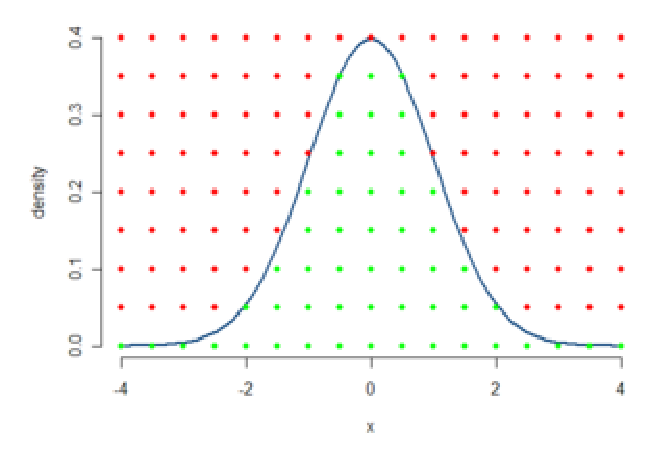
\includegraphics[width=\linewidth]{imgs/NormalRejectGrid.eps}
		\end{minipage}
		
	\end{frame}
	
	\begin{frame}
		\frametitle{Particular cases}
		
		Sometimes, we can benefit of mathematical transformations.\\
		The main weakness is that they are seldom compatible with variance
		reduction techniques.
		
		\mbox{}
		
		{\blue Example}: Box-Muller method for the normal law.
		
		\mbox{}
		
		{\red Idea}: it is easier to generate a point $(X, Y)$ from the bivariate
		normal law, of density on $\rit^2$
		\[
		f (x, y ) = \frac{1}{2\pi} e^{-(x^2 +y^2 )/2}.
		\]
		We change the cartesian coordinates $(X,Y)$ by the polar coordinates $(R, \Theta)$:\\
		\[
		R^2 = X^2 + Y^2 ; Y = R \sin \Theta.
		\]
		
		It gives an elegant approach, but incompatible with variance reduction techniques and can be slower than inversion.
		
\end{frame}

\begin{frame}
\frametitle{Box-Muller Algorithm}

\begin{enumerate}
\item
Independently draw $U_1$, $U_2$ from a $U(0,1)$ distribution.
\item
Set
\begin{align*}
R &= \sqrt{-2 \log (U_1)} \\
\theta &= 2 \pi U_2
\end{align*}
\item
Set
\begin{align*}
X &= R \cos(\theta) \\
Y &= R \sin(\theta)
\end{align*}
\end{enumerate}
		
\end{frame}

\begin{frame}
\frametitle{Multivariate distributions}

What if we want to draw from $\bsX: \Omega \rightarrow \calX \subseteq \RR^d$?

General approach:
\begin{itemize}
	\item Generate the marginals
	\item Combine the marginals as desired.
\end{itemize}
		
\end{frame}

\begin{frame}
\frametitle{Multivariate distributions: simple cases}

\begin{itemize}
\item 
Ideally, we can explicitly transform the marginals.
\item
Example: multivariate normal $\bsX \sim \calN(\bsmu, \Sigma)$, with
$$
\bsmu =
\begin{pmatrix}
	\mu_1 \\ \mu_2 \\ \vdots \\ \mu_d
\end{pmatrix}
\qquad
\Sigma = 
\begin{pmatrix}
	\sigma^2_1 & \sigma_{1,2} & \ldots & \sigma_{1,d} \\
	\sigma_{1,2} & \sigma^2_2 & \ldots & \sigma_{2,d} \\
	\vdots & \vdots & \ddots & \vdots \\
	\sigma_{1,d} & \sigma_{2,d} & \ldots & \sigma^2_d 
\end{pmatrix}
$$
Then,
$$
\bsX = \bsmu + L\calN(\bszero, \bsI)
$$
with $\Sigma = LL^T$, and $L$ is the Cholesky factor.

Drawing from $\calN(\bszero,\bsI)$: generate $d$ $\calN(0,1)$ independently.
\end{itemize}
		
\end{frame}

\begin{frame}
\frametitle{Multivariate distributions: copulae}

A $d$-variate \textcolor{red}{copula} $C: [0, 1]^d \rightarrow [0, 1] $is the cdf of a random vector
$(U_1,\ldots, U_d)$ with $U(0, 1)$ margins:
$$
C(u) = P[U_1 \leq u_1,\ldots, U_d \leq u_d]
$$
where
$$
P[U_j \leq u_j] = u_j
$$
for $j = 1,\ldots,d$, and $0 \leq u_j \leq 1$.

\end{frame}

\begin{frame}
\frametitle{Sklar's theorem}

\begin{theorem}[Sklar's theorem (1959)]
	\begin{itemize}
		\item 
	Let $H$ be a multivariate distribution function with margins $F_1,\ldots, F_d$.
	There exists a copula $C$ such that
$$
		H(x_1, \ldots, x_d) = C \left( F_1(x_1), \ldots, F_d(x_d) \right), \quad x_1, \ldots, x_d \in \overline{\RR}.
%		\label{eq:Copulas}
$$
	If $F_i$, $i = 1, \ldots, d$, are continuous then $C$ is unique. Otherwise $C$ is uniquely determined on the Cartesian product of the range of the marginals $F_1 \left( \overline{\RR} \right) \times \ldots \times F_d \left( \overline{\RR} \right)$.
	\item
	Conversely, if $C$ is a copula and $F_1, \ldots, F_d$ are univariate distribution functions, then the function $H$ defined above is a multivariate distribution function with margins $F_1, \ldots, F_d$.
	\end{itemize}
\end{theorem}

\end{frame}

\begin{frame}
\frametitle{Copula}

If we know the joint CDF $F$ and the marginals $F_1,\ldots,F_d$, we can find the copula via
$$
C(u_1,\ldots,u_d) = F\left(F_1^{-1}(u_1),\ldots,F_d^{-1}(u_d)\right),
$$
where $F_j^{-1}(\cdot)$ is the generalized inverse for margin $j$:
$$
F_j^{-1}(u) = \min \{ x \,:\, F_j(x) \geq u \}.
$$

\end{frame}

\begin{frame}
\frametitle{Fréchet–Hoeffding bounds}

Any bivariate copula $C$ verifies
$$
\max(F_X(x) + F_Y(y) - 1, 0) \leq C(x, y) \leq \min(F_X(x), F_Y(y))
$$

\mbox{}

\textcolor{blue}{Upper bound proof}
	\begin{align*}
		C(x, y) &= P[X \leq x \cap Y \leq y] \\ & \leq P[X \leq x] P[Y \leq y] \\ & \leq \min(F_X(x), F_Y(y))
	\end{align*}

\end{frame}

\begin{frame}
\frametitle{Fréchet–Hoeffding bounds}

\textcolor{blue}{Lower bound proof}
\begin{align*}
1 - C(x,y) &= P[X > x \cup Y > y] \\
& \leq P[X > x] + P[Y > y] \\
& = 1 - F_X(x) + 1 - F_Y(y)
\end{align*}
Thus,
$$
C(x,y) \geq F_X(x) + F_Y(y) - 1.
$$

\mbox{}

\textcolor{red}{Note:} this can be viewed as a particular of the Bonferroni inequality
$$
P \left[ \cap_{i = 1}^d A_i \right] \geq 1-d+\sum_{i = 1}^d P [A_i].
$$

\end{frame}

\begin{frame}
\frametitle{Gaussian copula}

$$
	C \left( F_1(x_1), \ldots, F_d(x_d) \right)
	= \Phi_{\Sigma} \left( \phi^{-1} \left( F_1(x_1) \right),\ldots, \phi^{-1}\left( F_d(x_d) \right) \right),
$$
where
\begin{itemize}
	\item $\phi$ is the cdf of a $\calN(0,1)$,
	\item $\Phi_{\Sigma}$ is the cdf of a $d$-dimensional $\calN(\bszero,\Sigma)$.
\end{itemize}

\end{frame}

\begin{frame}
\frametitle{Copulae estimation}

\begin{itemize}
	\item Parametric estimation;
	\item Non-parametric estimation;
	\item Machine-learning models (see Jutras et al.: \url{https://arxiv.org/abs/2302.09193v3}).
\end{itemize}

\end{frame}
	
\end{document}